\documentclass[10pt,a4paper,twocolumn]{article}
\usepackage[utf8]{inputenc}
\usepackage[english]{babel}
\usepackage{amsmath}
\usepackage{amsfonts}
\usepackage{amssymb}
\usepackage{graphicx}
\author{Håkan Ardö, Oleksiy Guzhva, Mikael Nilsson}
\title{Cow interaction watch dog}
\begin{document}
\maketitle

\begin{abstract}
Cows are interacting...
\end{abstract}

\section{Introduction}

Scientists working with animal behaviour and welfare are interested in studying the social interactions between cows in dairy farms. Typically that is performed by defining a set of interactions or events such as head butting, body pushing, social licking etc. and writing a very detailed protocol with the description of every event. Then an expert studies the area of interest for a large amount of time and counts the number of each behavioural event occuring for the whole duration of the video sequence/sequences used for the particular study \cite{MartinandBateson2007}. Some of these behavioural events are quite rare, which means that a lot of expert time have to be spent in looking at raw video data in order to find potentially interesting sequences that could be used for further annotations.

In this paper the goal is to take the first step towards an automated system for behavioral analysis. The study area is filmed using video cameras. Then an automated watchdog system will remove irrelevant parts (e.g. those, containing events that are not relevant or without animals in the scene) of the recorded video material. The remaining video sequences will still have to be studied by experts, but the time spent looking at uninteresting video sequences will be significantly reduced.

The pilot study used to develop this watchdog was made in a dairy barn in the south of Sweden with 252 Swedish Holstein cows. Cows were milked by four automatic milking robots, which had a common waiting area (6x18 meters). This waiting area is an common space which cows that are ready for milking could enter at any point in time. They will then interact with each other  in order to decide who are allowed to enter each of the milking robots and in which order. These interactions, their number and ratio between positive and negative behavioural events are highly dependent on cow's rank in a herd hierarchy. There are studies showing the correlation between subtle changes in animal behaviour and their health or their welfare. Therefore, studies explaining the social component of animal behaviour are of great importance as they could help in avoiding unnecessary aggression between animals and improve their being.

Video recordings were made using three Axis M3006-V cameras with a wide angle of 134 degrees that were placed at 3.6 meter height, pointing straight down to optimize overview over the study area. There is a significant overlap between the camera images in order to not miss events taking place at the border between the cameras. In total 2315 hours (1 month) of 800x600 video in 16 Frames Per Second (FPS), RGB colour space, was collected.

The cameras were calibrated to compensate for lens distortion and rectification. Although the cameras were physically mounted to point fairly straight down, they were still slightly tilted. This tilting was synthetically removed during the rectification. The end result of this calibration is video images where the cows have the same size regardless of where in the image they appear. Also the scan-lines of the three different cameras become aligned, which allows them to be stitched together to form an overview of the entire waiting area.

Finally a Convolution Neural Network (CNN)  was trained to detect the cows in the images, and statistics about how many cows and their distances/relation to each other was extracted. Using the statistical data, scientists working in a field of animal behaviour could form queries to select particular time intervals to watch, such as "show me video clips involving at least two cows with the neck of one cow closer than one meter to the body of the other".

\section{Brief technical about calibration approach?}

FIXME: I'm afard I've used the old calibration here...

In order to fulfil the specific research questions regarding dairy barn slatted floor and distribution of animals on it,
correct transition of image coordinates into real-world coordinates was crucial. To assure that all the coordinates
can be reliable and that the observer/algorithm will be able to correctly identify all the objects, three images were
merged and synchronized after applying normalization algorithms. Setups with only one camera (even with wide
observation angle) could suffer from a number of image artefacts (e.g. radial distortion, tangential distortion,
occlusion between objects/cows) therefore; it was decided to use three cameras for a relatively small region of
interest (ROI) in the waiting area.

For this study, the classical pinhole camera model augmented with a lens distortion model was used for scene view
reconstruction. The scene view was formed through the projection of 3D world points into the image
plane and to assure correct disposition and perspective of objects in a merged image covering the ROI, we used
number of planar markers to estimate scene homography and lens distortion. The camera calibration method
developed by Tsai (1986) and further improved by Horn (2000) includes both interior and exterior orientations,
corrections for the distortion and a scale factor for the reliable correlation between target and scene coordinates.
The number of planar markers was used for the camera calibration on site (Figure 1). These markers were placed
at the height of the virtual floor. This height was estimated to be 1.49 meters with a standard deviation of 0.05 by
measuring twelve random cows in the study area.

\section{CNN cow detector}

A random subset of the full recording consisting of 1722 images was manually annotated. This subset contained in total 6399 cows. Each cow was annotated with seven landmark points: head, left and right shoulder, front middle, left and right hip and back middle. In addition to that one additional landmark "cow center" was defined as the mean of front middle and back middle. This data was then used to train a CNN detector.

The detector was split into two step. The first step is a fully convolutional CNN that detects the landmarks in the image. Currently only four of the landmarks were used to speed up the experiments, but extending to use all 8 is straight forward. The architecture of this network is a fully convolutional version of VGG \cite{Simonyan14c} with batch normalization \cite{DBLP:journals/corr/IoffeS15} added after each convolution step. Details are shown in Table \ref{tab:cownet}.

The second step is another CNN that works with the probability map produced by the first as input and tries to detect the cows and their orientations. The full circle is divided into 32 equally spaced orientations which generates 32 different oriented cow classes. In addition to that there is the no cow class, which makes the total number of classes of this CNN 33. The input probabilities was turned into log likelihoods as it makes more sense when summing them together. Then the network consists of a single $ 13 \times 13 $ convolutional layer. Details are shown in Table \ref{tab:cowdirnet}.

\begin{table}
\begin{center}
\begin{tabular}{|l|c|c|}
\hline
\textbf{Layer type} & \textbf{Size} & \textbf{Channels} \\
\hline

Conv + BNorm + Relu & 3x3 & 32 \\
MaxPool(stride=2) & 2x2 &  \\
\hline

Conv + BNorm + Relu & 3x3 & 64 \\
MaxPool(stride=2) & 2x2 &  \\
\hline

Conv + BNorm + Relu & 3x3 & 128 \\
Conv + BNorm + Relu & 3x3 & 128 \\
MaxPool(stride=2) & 2x2 &  \\
\hline

Conv + BNorm + Relu & 3x3 & 256 \\
Conv + BNorm + Relu & 3x3 & 256 \\
MaxPool(stride=2) & 2x2 &  \\
\hline

Conv + BNorm + Relu & 3x3 & 512 \\
Conv + BNorm + Relu & 3x3 & 512 \\
MaxPool(stride=2) & 2x2 &  \\
\hline

Conv + BNorm + Relu & 1x1 & 1024 \\
Conv + BNorm + Relu & 1x1 & 1024 \\
Conv + BNorm + Relu & 1x1 & 5 \\
Softmax & & \\
\hline

\end{tabular}
\end{center}
\caption{CNN architecture used to detect different landmarks of the cows. The input is an image of any size with 3 rgb channels scaled to the range $\left[0,\,1\right]$. The output is probability map segmenting the entire image into 5 classes: Ground, Cow front middle, Cow center, Cow back middle and Cow head.}
\label{tab:cownet}
\end{table}

\begin{table}
\begin{center}
\begin{tabular}{|l|c|c|}
\hline
\textbf{Layer type} & \textbf{Size} & \textbf{Channels} \\
\hline

MaxPool(stride=1) & 3x3 &  \\
Log & & \\
Conv + BNorm + Relu & 13x13 & 33 \\
Softmax & & \\
\hline
\end{tabular}
\end{center}
\caption{CNN architecture use to detect the cows and their orientation. The input is the 5 channel probability map from the landmark detector with the last MaxPool removed to increase resolution. The output is a probability map that segments the image into either background or cow in one of 32 different orientations.}
\label{tab:cowdirnet}
\end{table}

The landmark net were trained on patches of $150\times 150$ pixels extracted from the input images. This makes the output during training a single pixel. The positive examples were centred on the landmarks and randomly jittered $\pm 16$ pixels (as the distance between output pixels is $32$ input pixels). Negative patches where selected at centres more than $32$ pixels from any landmark. In addition to the positive and negative patches a set of don't care patches were selected at random centres at distances between $16$ and $32$ pixels from landmarks. The ground truth probability of these patches belong to the class of the landmark was set to $0.5$ and the probability that they are ground was set to $0.5$. In some cases several landmarks appears within $32$ pixels of the patch center. In that case the probability mass was distributed uniformly among all involved classes.

The weights of the convolutions are initiated using random samples draw from a Gaussian
distribution truncated at $2\sigma$, with standard deviation $\sigma=\sqrt{\frac{2}{n}}$,
where $n$ is the number of inputs\cite{DBLP:journals/corr/HeZR015}. The networks are regularized with weight decay of
$0.0001$ and optimized using stochastic gradient descent with $0.9$ momentum. The
learning rate is initiated to $1.0$ and reduced by a factor $10$ each time the validation
error flattens. The landmark CNN uses only valid outputs from the convolutional and maxpool
layers while the cow detector keeps the same resolution to also detect cows that are
slightly outside the image.

Once the net was trained, the last maxpool layer was removed to increase the output resolution. The net was then applied to the full rectified training images producing probability maps of $44\times 46\times 5$ pixels. These were used as training examples for the cow detection net (without splitting them into patches). Output ground truth probability maps of $44\times 46\times 33$ pixels were constructed from the annotations by projecting each cow, $i$, center point into the probability map as $\left( x_i, y_i \right)$ and calculate its angle $a_i$ as the angle of line between front middle and back middle. Then a binary $44\times 46\times 33$ mask $B\left( x, y, c \right)$ is formed, containing a background mask
\begin{equation}
B\left( x, y, 32 \right) = \left\lbrace
\begin{array}{clc}
0 & \text{if} &
\begin{array}{c}
 \lfloor x_i \rfloor \leq x \leq \lceil x_i \rceil \\
 \lfloor y_i \rfloor \leq y \leq \lceil y_i \rceil
\end{array}
\\
1 & \multicolumn{2}{l}{\text{otherwise}}
\end{array}
\right.
\end{equation}
and $32$ orientation masks
\begin{equation}
B\left( x, y, c \right) = \left\lbrace
\begin{array}{clc}
1 & \text{if} &
\begin{array}{c}
 \lfloor x_i \rfloor-1 \leq x \leq \lceil x_i \rceil+1 \\
 \lfloor y_i \rfloor-1 \leq y \leq \lceil y_i \rceil+1 \\
 \mathrm{adist}\left(\frac{2c\pi}{32}, c_i\right) < \frac{2\pi}{32} \\
\end{array}
\\
0 & \multicolumn{2}{l}{\text{otherwise}}
\end{array}
\right.
\end{equation}
for $0\leq c \leq 31$ and all $i$. The $\mathrm{adist}$ function calculates the absolute angular distance between two angles. The ground truth probability masks are then produced by normalising $B$ to sum to $1$ for each pixel. Finally, the network is trained using the same hyper parameters as described above.


\begin{figure*}[tb]
\begin{center}
  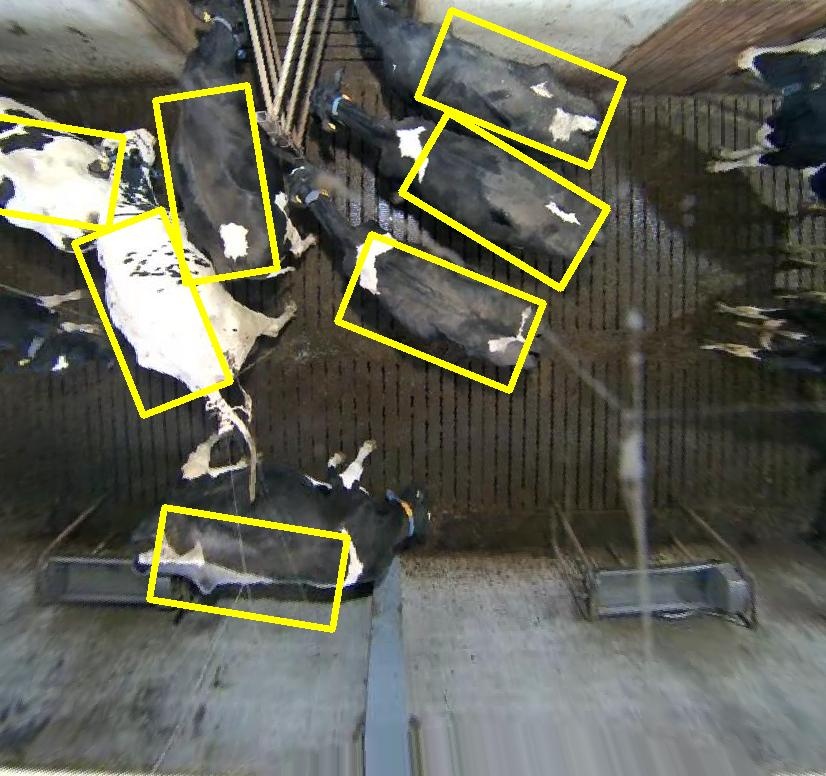
\includegraphics[width=0.3\textwidth]{ok/1419422172315416.jpg}
  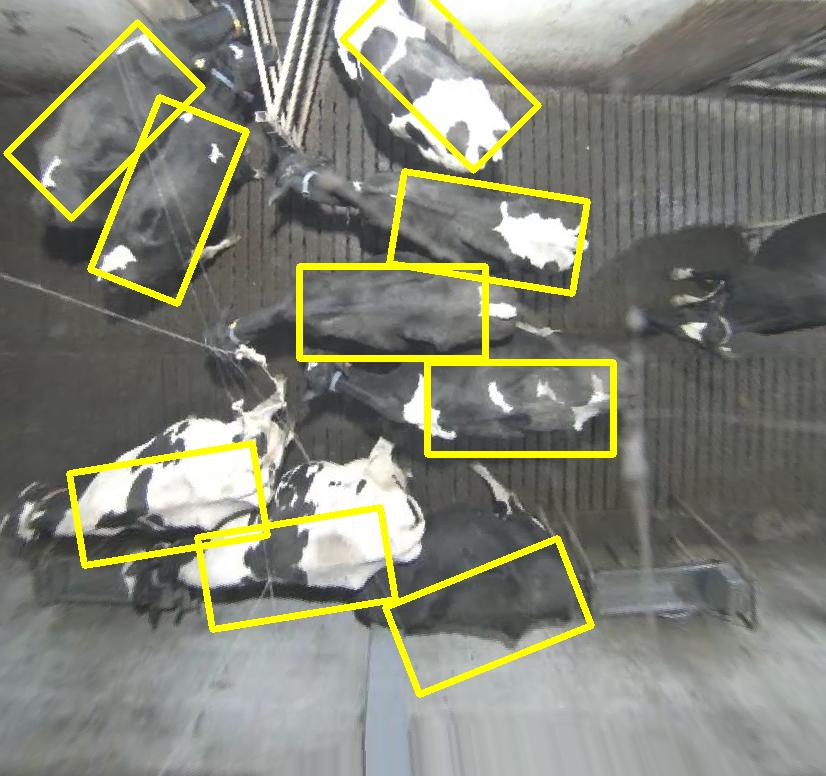
\includegraphics[width=0.3\textwidth]{ok/1419630968631761.jpg}
  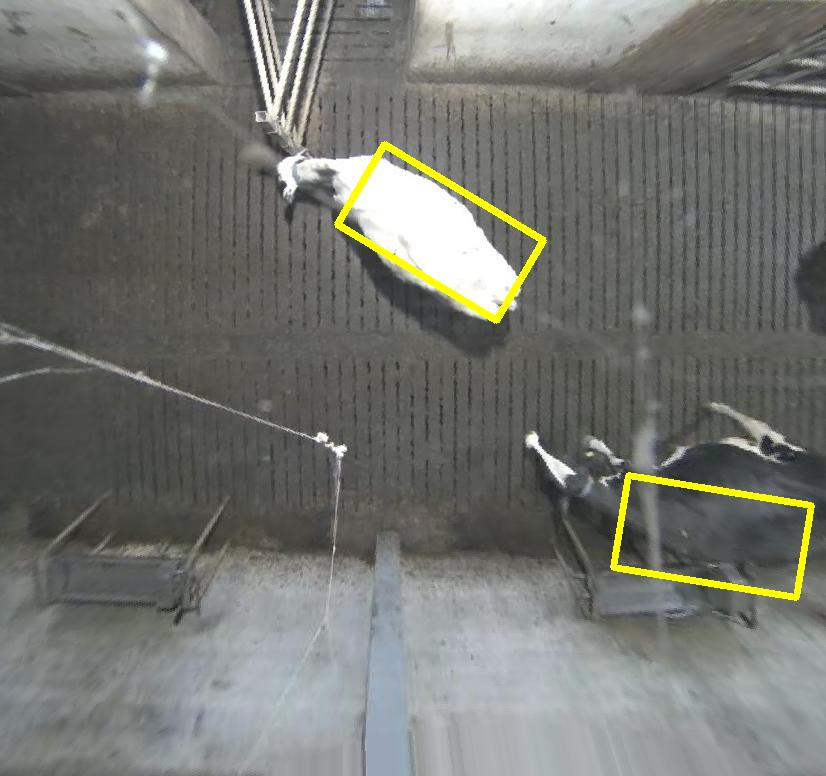
\includegraphics[width=0.3\textwidth]{ok/1420251135794580.jpg}

\vspace{1mm}

  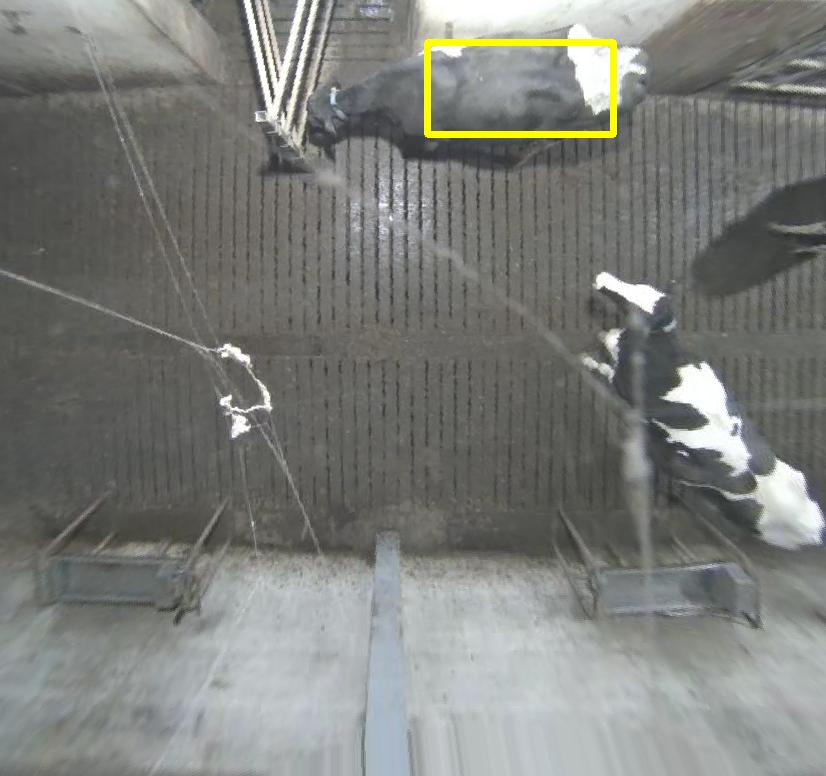
\includegraphics[width=0.3\textwidth]{bad/1419743355933936.jpg}
  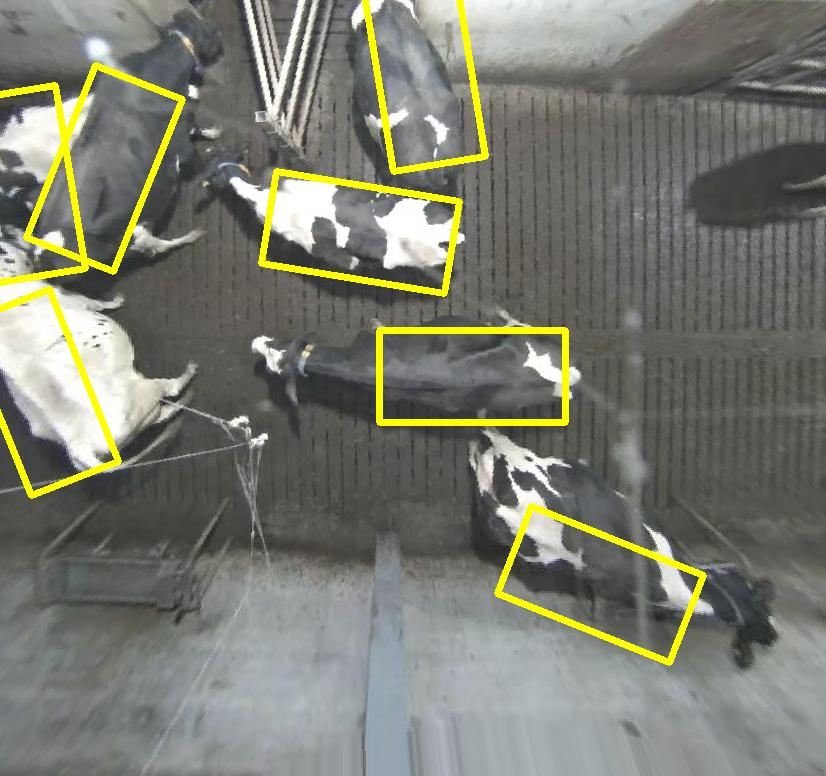
\includegraphics[width=0.3\textwidth]{bad/1420050868326145.jpg}
  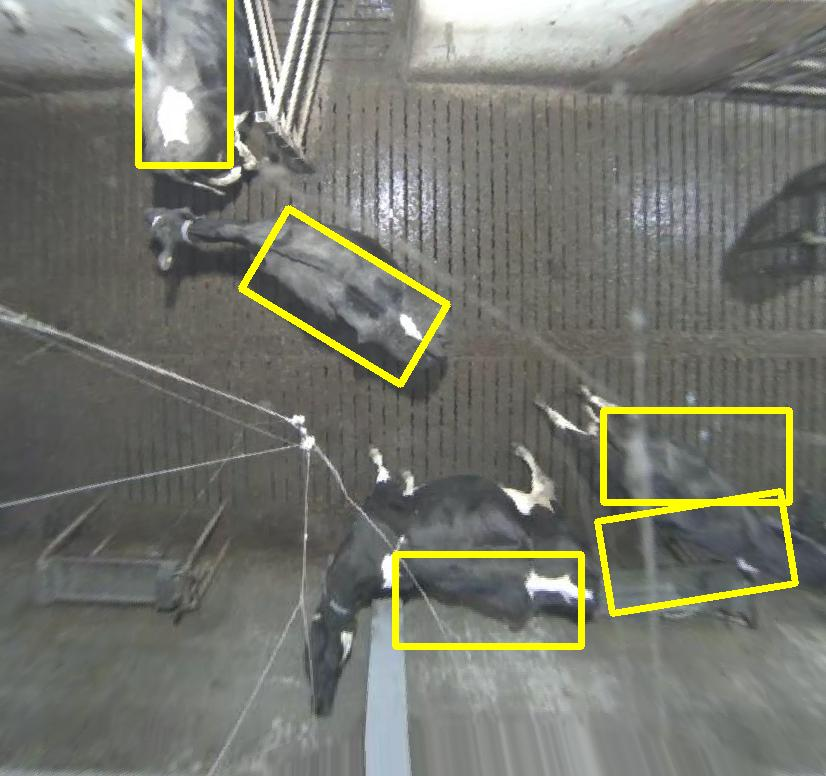
\includegraphics[width=0.3\textwidth]{bad/1420185482574217.jpg}
\end{center}
  \caption{Results from the evaluation. Top row: Three images correctly interpretated (all cows detected and no extra detections). Bottom row: The three images were the errors were made (1 missed cow and two extra detections).}
  \label{fig:res}
\end{figure*}

\section{Watchdog evaluation}
To evaluate the system, the 6400 frames spread over the entire recording were processed by the CNN. A simple watchdog extracting frames containing two or more cows were implemented. That would be the most basic requirement for an interaction, and already with this simple criteria it was possible to discard 38 \% of the recordings as uninteresting. 50 random frames selected by the watchdog and 50 random frames discarded by the watchdog were automatically annotated by using the CNN results and studied manually. Cows intersecting the borders were ignored in the sens that the images was considered correct regardless of wheter such border cases was detected or not.

97 \% of the images were perfectly interpretated, i.e. all cows present were detected and no extra detections. Two of the images with errors containd several detected cows and was thus correcly classified as containing two or more cows by the watchdog, resuting in a watchdog-hitrate for it of 99 \%. In totalt those 100 images contains 222 cows. One of those were not detected and 2 extra detections were made yielding a cow-hitrate of 99.6 \% with a false alarm rate of 0.9\%.

\section{Conclusions}

\bibliographystyle{plain}
\bibliography{main}

\end{document}
